\documentclass{article}

% ready for submission
\usepackage[preprint]{neurips_2026}

\usepackage[utf8]{inputenc}
\usepackage[T1]{fontenc}
\usepackage{hyperref}
\usepackage{url}
\usepackage{booktabs}
\usepackage{amsfonts}
\usepackage{nicefrac}
\usepackage{microtype}
\usepackage{xcolor}
\usepackage{amsmath}
\usepackage{amssymb}
\usepackage{graphicx}

\raggedbottom

\title{Training-Efficient Physics-Informed Neural Networks for Incompressible Laminar Flow Around a Cylinder}

\author{%
  Chi-Han Chiu, Chen-Yan Juang, Ming-Yang Wu, and Jing-Hua Chang (Team 12) \\
  Department of Electrical and Computer Engineering\\
  University of California San Diego\\
  \texttt{\{c8chiu, chjuang, miw090, jic184\}@ucsd.edu}
}

\begin{document}

\maketitle

\begin{abstract}
Physics-informed neural networks (PINNs) provide a mesh-free way to learn continuous flow fields while enforcing governing equations through residual losses. We reproduce and extend the mixed-variable PINN of Rao et al. for two-dimensional incompressible laminar flow around a cylinder at $Re=10$. Against a Chorin projection reference solution, our reproduction obtains post-initial-transient mean relative $L_2$ errors of 5.30\%, 19.86\%, and 10.79\% for $u$, $v$, and $p$, respectively. We then study training-side directions: a GPU-resident L-BFGS backend, residual-aware adaptive collocation, and causal loss scheduling. The GPU-resident backend achieves a $1.23\times$ speedup and 11.0\% lower estimated energy while maintaining comparable accuracy. Causality-weighted Adam pretraining followed by unweighted L-BFGS polish gives the best tested post-initial-transient mean relative $L_2$ errors of 4.64\%, 18.60\%, and 8.89\%. Overall, the completed quantitative results indicate that optimizer implementation and loss scheduling are critical to PINN efficiency and stability; adaptive collocation remains a promising sampling direction that should be validated with fixed-grid error metrics. We additionally outline two exploratory directions, alternative network architectures and a three-dimensional extension, as preliminary work.
\end{abstract}

\section{Introduction}

Fluid dynamics is governed by nonlinear partial differential equations whose solutions are central to engineering design, aerodynamics, biomedical devices, and industrial systems. Traditional numerical solvers such as finite-volume and finite-element methods remain the standard tools for high-fidelity simulation. However, they often require mesh generation, repeated linear or nonlinear solves, and substantial computational cost, especially when many parameter sweeps or repeated queries are needed. Purely data-driven neural networks can approximate flow fields from examples, but they may produce physically inconsistent solutions and usually require dense labeled simulation data.

Physics-informed neural networks (PINNs) address a different point in this design space. Rather than replacing high-fidelity computational fluid dynamics (CFD), PINNs provide a differentiable, continuous field representation whose training objective includes governing equations, boundary conditions, and initial conditions through automatic differentiation~\cite{raissi2019pinn,karniadakis2021pinnreview}. This makes them attractive for data-scarce settings, inverse or partially observed problems, and repeated-query surrogate modeling. Their practical performance, however, is limited by optimization difficulty, collocation-point allocation, imbalance between PDE, boundary-condition, and initial-condition loss terms, and implementation overhead.

This project studies these issues using the incompressible laminar cylinder-flow benchmark from Rao et al.~\cite{rao2020pinnflow}. We reproduce the mixed-variable PINN formulation, validate it against a Chorin projection reference solver, and investigate training improvements along three practical dimensions: backend efficiency, adaptive collocation, and temporal loss scheduling. Our contributions are:
\begin{itemize}
    \item We reproduce the mixed-variable PINN benchmark for $Re=10$ incompressible cylinder flow and evaluate the learned $u$, $v$, and $p$ fields against a Chorin projection reference solution.
    \item We implement and benchmark a GPU-resident L-BFGS training backend that improves wall-clock time, per-evaluation latency, estimated energy, and GPU utilization while preserving comparable accuracy.
    \item We evaluate causality-weighted Adam pretraining quantitatively and investigate residual-aware adaptive collocation as a preliminary sampling strategy. The completed results show that loss scheduling provides the clearest measured accuracy improvement in our experiments.
\end{itemize}
Beyond these three validated directions, we also include preliminary discussions of two exploratory extensions, alternative network architectures and a three-dimensional generalization, which we report as work in progress rather than as quantitatively validated results.

\section{Related Work}

\paragraph{Physics-informed neural networks.}
Raissi et al.~\cite{raissi2019pinn} introduced PINNs as a framework for solving forward and inverse PDE problems by embedding differential-equation residuals into neural network training. Karniadakis et al.~\cite{karniadakis2021pinnreview} surveyed PINNs as a broader scientific machine-learning paradigm. Compared with conventional supervised surrogates, PINNs reduce the need for dense labeled solution fields by using the physical residual itself as a training signal.

\paragraph{PINNs for incompressible flow.}
Rao et al.~\cite{rao2020pinnflow} proposed a mixed-variable PINN formulation for incompressible laminar flow, using a stream function and stress variables to improve constraint satisfaction. This formulation is especially useful for two-dimensional incompressible flow because the stream function enforces the continuity equation by construction. Our reproduction follows this mixed-variable formulation and uses it as the baseline for evaluating training improvements.

\paragraph{Training and sampling challenges.}
Despite their flexibility, PINNs often suffer from optimization imbalance, spectral bias, and inefficient collocation usage. Fixed random collocation may spend training budget on regions that already satisfy the PDE while under-sampling regions with larger residuals. Residual-based adaptive sampling addresses this issue by reallocating collocation points during training. Temporal causality weighting further improves transient-flow training by encouraging earlier time segments to be learned before later segments~\cite{wang2024causal}. These observations motivate our focus on training strategy rather than only model architecture.

\section{Problem Setup and PINN Formulation}

\subsection{Governing Equations and Benchmark}

We consider two-dimensional incompressible laminar flow around a circular cylinder in a rectangular channel. Let $\mathbf{u}=(u,v)$ denote velocity, $p$ pressure, $\rho$ density, and $\mu$ dynamic viscosity. In stress form, the incompressible Navier--Stokes equations are
\begin{align}
    \nabla \cdot \mathbf{u} &= 0, \\
    \frac{\partial \mathbf{u}}{\partial t} + (\mathbf{u}\cdot\nabla)\mathbf{u}
    &= \frac{1}{\rho}\nabla\cdot\boldsymbol{\sigma}, \\
    \boldsymbol{\sigma} &= -p\mathbf{I} + \mu\left(\nabla\mathbf{u}+\nabla\mathbf{u}^{T}\right),
\end{align}
where $\boldsymbol{\sigma}$ is the Cauchy stress tensor. Following the cylinder-flow setting used by Rao et al.~\cite{rao2020pinnflow} and related CFD benchmark definitions~\cite{schafer1996benchmark}, we evaluate the $Re=10$ case over $t\in[0,0.5]$~s. Although this is a low-Reynolds-number laminar case, the benchmark is time-dependent and is useful for evaluating transient PINN training behavior.

The reference solution is generated by a Chorin fractional-step projection method~\cite{chorin1968projection} on a uniform $220\times82$ grid with time step $\Delta t=0.001$~s. We use this reference to evaluate the learned velocity and pressure fields at multiple time snapshots. Pressure errors are reported with caution because pressure in incompressible flow is sensitive to the pressure gauge and to projection-step splitting error.

\subsection{Mixed-Variable PINN}

We use the mixed-variable PINN formulation from Rao et al.~\cite{rao2020pinnflow}. The neural network maps the spatiotemporal coordinate $(x,y,t)$ to five output fields:
\begin{equation}
    (x,y,t) \mapsto (\psi, p, \sigma_{11}, \sigma_{22}, \sigma_{12}),
\end{equation}
where $\psi$ is the stream function, $p$ is pressure, and $\sigma_{ij}$ are stress components. The velocity field is recovered from the stream function as
\begin{equation}
    u = \frac{\partial \psi}{\partial y}, \qquad
    v = -\frac{\partial \psi}{\partial x}.
\end{equation}
This construction satisfies incompressibility identically because
\begin{equation}
    \frac{\partial u}{\partial x} + \frac{\partial v}{\partial y}
    = \frac{\partial^2\psi}{\partial x\partial y}
    - \frac{\partial^2\psi}{\partial y\partial x} = 0.
\end{equation}

The PDE residual consists of momentum residuals, stress-constitutive residuals, and pressure--stress consistency. In compact form, the physical objective is
\begin{equation}
    \mathcal{L}
    = \mathcal{L}_{\mathrm{PDE}}
    + \lambda_{\mathrm{wall}}\mathcal{L}_{\mathrm{wall}}
    + \lambda_{\mathrm{inlet}}\mathcal{L}_{\mathrm{inlet}}
    + \lambda_{\mathrm{outlet}}\mathcal{L}_{\mathrm{outlet}}
    + \lambda_{\mathrm{ic}}\mathcal{L}_{\mathrm{ic}},
\end{equation}
where $\mathcal{L}_{\mathrm{PDE}}$ is the mean-squared residual over collocation points and the remaining terms enforce no-slip wall conditions, inlet velocity, outlet pressure, and the initial condition. We use fixed loss weights $\lambda_{\mathrm{wall}}=\lambda_{\mathrm{inlet}}=5$ and $\lambda_{\mathrm{outlet}}=\lambda_{\mathrm{ic}}=1$, with unit weight on $\mathcal{L}_{\mathrm{PDE}}$. All spatial and temporal derivatives are computed by automatic differentiation.

\subsection{Network and Training Configuration}
\label{sec:config}

The network is a fully-connected multilayer perceptron with seven hidden layers of $50$ units and $\tanh$ activations, mapping the three inputs $(x,y,t)$ to the five output fields $(\psi,p,\sigma_{11},\sigma_{22},\sigma_{12})$; weights are initialized with Xavier-normal initialization. The $Re=10$ regime is set by density $\rho=1.0$ and dynamic viscosity $\mu=0.005$, with a pulsatile inlet of period $1.0$~s over $t\in[0,0.5]$~s. Collocation points are drawn by Latin-hypercube sampling: $100{,}000$ points over the full domain, augmented with $15{,}000$ points refining the near-cylinder wake region and $3{,}000$ points along each of the two channel walls. Training uses Adam for $20{,}000$ iterations at a learning rate of $10^{-3}$, followed by an L-BFGS phase; the \emph{reproduce} baseline runs L-BFGS through SciPy L-BFGS-B, whereas the GPU-resident and causal runs use \texttt{torch.optim.LBFGS}. For causal weighting, the time domain is split into $M=32$ equal-duration temporal bins.

\section{Training Improvements}

\subsection{GPU-Resident L-BFGS Backend}

The reproduction baseline uses a SciPy L-BFGS-B optimization loop. This approach is straightforward but repeatedly passes flattened parameters, loss values, and gradients between the optimizer and the tensor framework. To reduce this overhead, we implement a GPU-resident training backend using \texttt{torch.optim.LBFGS}. In this implementation, model parameters, loss evaluation, and gradient computation remain on the GPU during each L-BFGS closure, reducing repeated host-device transfers. This modification changes only the execution backend; the PINN objective and evaluation protocol remain unchanged.

\subsection{Residual-Aware Adaptive Collocation}

\textcolor{red}{[\textbf{TODO (Ming-Yang Wu)}: describe the residual-aware adaptive collocation method.]}

\subsection{Temporal Causality and Loss Balancing}

For transient flows, treating time simply as another neural-network input may underuse the temporal ordering of the physical process. We therefore incorporate temporal-causality weighting~\cite{wang2024causal}. The time domain is partitioned into $M$ equal-duration bins (we use $M=32$; see Section~\ref{sec:config}), and the loss for bin $i$ is weighted by
\begin{equation}
    w_i = \exp\left(-\frac{\epsilon}{M}\sum_{k<i}L_k\right),
\end{equation}
where $L_k$ is the residual loss of an earlier time bin and the summation is treated as a stop-gradient term. When $\epsilon=0$, all weights become one and the objective reduces to the standard unweighted residual; the GPU-resident run optimizes exactly this unweighted objective and therefore serves as our $\epsilon=0$ reference, so we do not run a separate $\epsilon=0$ ablation. We evaluate two strategies: keeping causal weights fixed during L-BFGS (\emph{frozen}) and switching back to the unweighted physical loss during L-BFGS (\emph{uniform}).

We also consider adaptive loss weighting to reduce competition between PDE residuals and boundary-condition terms. However, preliminary gradient-norm and neural-tangent-kernel-based loss-balancing variants did not yield measurable field-$L_2$ improvements in our setting, and some configurations drifted toward a trivial near-zero-flow solution; we report these as negative results. In this report, the most complete quantitative results come from causality-weighted Adam pretraining and backend-efficiency experiments. Adaptive collocation, adaptive loss weighting, and architecture variants are therefore treated as partially validated directions unless additional fixed-grid $L_2$ results are included.

\section{Results and Analysis}

\subsection{Evaluation Metrics}
\label{sec:metrics}

For each scalar field $q\in\{u,v,p\}$, the relative $L_2$ error is defined as
\begin{equation}
    \varepsilon_q
    = \frac{\|q_{\mathrm{pred}} - q_{\mathrm{ref}}\|_2}
           {\|q_{\mathrm{ref}}\|_2}.
\end{equation}
We report errors as percentages. \emph{Mean} $L_2$ is computed by averaging per-snapshot errors over all evaluated post-initial-transient snapshots with $t\geq0.1$~s. \emph{Global} $L_2$ is computed after stacking all evaluated snapshots into a single vector. These two metrics can differ because averaging per-snapshot ratios is not equivalent to taking one ratio over the full trajectory. For pressure, both predicted and reference fields are spatially demeaned at each snapshot before computing $\varepsilon_p$, removing the arbitrary additive pressure gauge.

\subsection{Baseline Reproduction and Backend Efficiency}

The reproduction baseline and the GPU-resident backend reach comparable post-initial-transient accuracy (mean $L_2$ errors summarized in Table~\ref{tab:l2_causal}): the GPU-resident run shows slightly larger velocity errors but a slightly smaller mean pressure error. Pressure is the least stable field---for example, near $t=0.5$~s the per-snapshot pressure error rises above 60\%---reflecting the gauge sensitivity of projection-based incompressible-flow references.

% --- C1: per-snapshot table commented out to compress length. Mean values are
% retained in Table~\ref{tab:l2_causal}; the only unique datum (the t=0.5 s
% pressure spike) is now stated in the text above. Uncomment to restore. ---
\iffalse
\begin{table}[h]
  \caption{Selected per-snapshot $L_2$ relative error (\%) for $Re=10$. \emph{reproduce} is the SciPy L-BFGS-B baseline; \emph{GPU-resident} is the PyTorch L-BFGS run. The mean is computed over all 41 post-initial-transient snapshots with $t\geq0.1$~s.}
  \label{tab:l2_snapshots}
  \centering
  \resizebox{0.55\textwidth}{!}{%
  \begin{tabular}{@{}c ccc ccc@{}}
    \toprule
    & \multicolumn{3}{c}{reproduce} & \multicolumn{3}{c}{GPU-resident} \\
    \cmidrule(lr){2-4}\cmidrule(lr){5-7}
    $t$ (s) & $\varepsilon_u$ & $\varepsilon_v$ & $\varepsilon_p$
            & $\varepsilon_u$ & $\varepsilon_v$ & $\varepsilon_p$ \\
    \midrule
    0.10 & 10.19 & 41.74 &  3.44 & 11.87 & 47.50 &  2.42 \\
    0.20 &  5.63 & 24.39 &  4.29 &  6.77 & 27.27 &  4.23 \\
    0.30 &  4.25 & 16.47 &  9.06 &  4.93 & 18.61 &  9.04 \\
    0.40 &  4.44 & 13.29 &  4.45 &  4.50 & 14.70 &  6.33 \\
    0.50 &  4.81 & 12.60 & 70.08 &  4.72 & 13.57 & 63.86 \\
    \midrule
    Mean & \textbf{5.30} & \textbf{19.86} & 10.79 & 5.94 & 22.23 & \textbf{10.31} \\
    \bottomrule
  \end{tabular}}
\end{table}
\fi

Table~\ref{tab:backend_bench} shows that the GPU-resident backend improves computational efficiency. For 1000 L-BFGS function evaluations on one RTX 3090, it achieves a $1.23\times$ speedup, 18.6\% lower per-evaluation latency, 11.0\% lower estimated energy, and 14 percentage points higher mean GPU utilization.

\begin{table}[h]
  \centering
  \caption{Backend benchmark: 1000 L-BFGS function evaluations on one RTX 3090. Energy is estimated as mean GPU power draw multiplied by wall-clock time.}
  \label{tab:backend_bench}
  \resizebox{0.6\textwidth}{!}{%
  \begin{tabular}{@{}lccc@{}}
    \toprule
    Metric & reproduce & GPU-resident & Change \\
    \midrule
    Wall time       & $204.1$\,s & $\mathbf{166.4}$\,s & $1.23\times$ faster \\
    Eval latency    & $204$\,ms  & $\mathbf{166}$\,ms  & $18.6\%$ lower \\
    Energy          & $59.8$\,kJ & $\mathbf{53.2}$\,kJ & $11.0\%$ lower \\
    GPU utilization & $68\%$     & $\mathbf{82\%}$     & $+14$ pp \\
    \bottomrule
  \end{tabular}}
\end{table}


\subsection{Adaptive Collocation Behavior}

\textcolor{red}{[\textbf{TODO (Ming-Yang Wu)}: report the adaptive-collocation results.]}

\subsection{Causal Training Performance}

Table~\ref{tab:l2_causal} compares the reproduction baseline, GPU-resident backend, and causal training variants. The ``Loss'' column is the final training objective value for each run and should be interpreted together with the $L_2$ metrics because causal and uniform phases use different loss schedules. Causality-weighted Adam pretraining followed by an unweighted L-BFGS polish achieves the lowest error among the tested configurations. The best configuration is causal $\epsilon=30$ with unweighted L-BFGS polish, which achieves mean relative $L_2$ errors of 4.64\%, 18.60\%, and 8.89\% for $u$, $v$, and $p$. Figure~\ref{fig:field_comparison} shows the predicted and reference $u$, $v$, and $p$ fields for this configuration at $t=0.5$~s; the velocity fields match closely and the demeaned pressure recovers the correct large-scale structure.

\begin{table*}[h]
  \centering
  \caption{$Re=10$ post-initial-transient error ($t\geq0.1$~s). \emph{frozen} keeps causal weights during L-BFGS; \emph{uniform} switches back to the unweighted physical loss during L-BFGS.}
  \label{tab:l2_causal}
  \resizebox{0.85\textwidth}{!}{%
  \begin{tabular}{@{}l c ccc ccc@{}}
    \toprule
    & & \multicolumn{3}{c}{Mean $L_2$ (\%)} & \multicolumn{3}{c}{Global $L_2$ (\%)} \\
    \cmidrule(lr){3-5}\cmidrule(lr){6-8}
    Run & Loss & $\varepsilon_u$ & $\varepsilon_v$ & $\varepsilon_p$
        & $\varepsilon_u$ & $\varepsilon_v$ & $\varepsilon_p$ \\
    \midrule
    reproduce (baseline) & $2.10{\times}10^{-4}$ & 5.30 & 19.86 & 10.79 & 4.47 & 14.75 & 27.92 \\
    GPU-resident         & $2.94{\times}10^{-3}$ & 5.94 & 22.23 & 10.31 & 4.75 & 16.44 & 24.42 \\
    \midrule
    causal $\epsilon{=}30$, frozen  & $2.31{\times}10^{-4}$ & 5.22 & 20.38 & 11.03 & 4.36 & 15.02 & 28.49 \\
    causal $\epsilon{=}30$, uniform & $\mathbf{1.53{\times}10^{-4}}$ & \textbf{4.64} & \textbf{18.60} & \textbf{8.89} & \textbf{3.93} & \textbf{13.28} & \textbf{22.51} \\
    causal $\epsilon{=}50$, frozen  & $2.11{\times}10^{-4}$ & 5.34 & 19.86 & 10.10 & 4.47 & 15.05 & 25.83 \\
    causal $\epsilon{=}50$, uniform & $1.54{\times}10^{-4}$ & 4.96 & 19.21 & 9.70 & 4.14 & 13.93 & 25.30 \\
    \bottomrule
  \end{tabular}}
\end{table*}

The comparison between \emph{frozen} and \emph{uniform} L-BFGS suggests that causal weighting is most useful as an initialization mechanism during Adam training. Keeping causal weights frozen during L-BFGS can bias the optimizer toward earlier time bins, while switching back to the unweighted physical loss allows L-BFGS to polish the full trajectory. This supports a two-stage interpretation: causal weighting improves the training path, but the final model should be optimized against the original unweighted physical objective. As shown in Figure~\ref{fig:causal_weight}, the minimum causal weight $\min_i w_i$ rises gradually over Adam training but saturates near $0.84$ ($\epsilon=30$) and $0.77$ ($\epsilon=50$), indicating that the curriculum does not fully reach the latest time bins within the iteration budget; this is consistent with $\epsilon=30$ and $\epsilon=50$ converging to nearly identical accuracy. The corresponding unweighted training-loss trajectories are shown in Figure~\ref{fig:loss_curves}.

\begin{figure}[h]
  \centering
  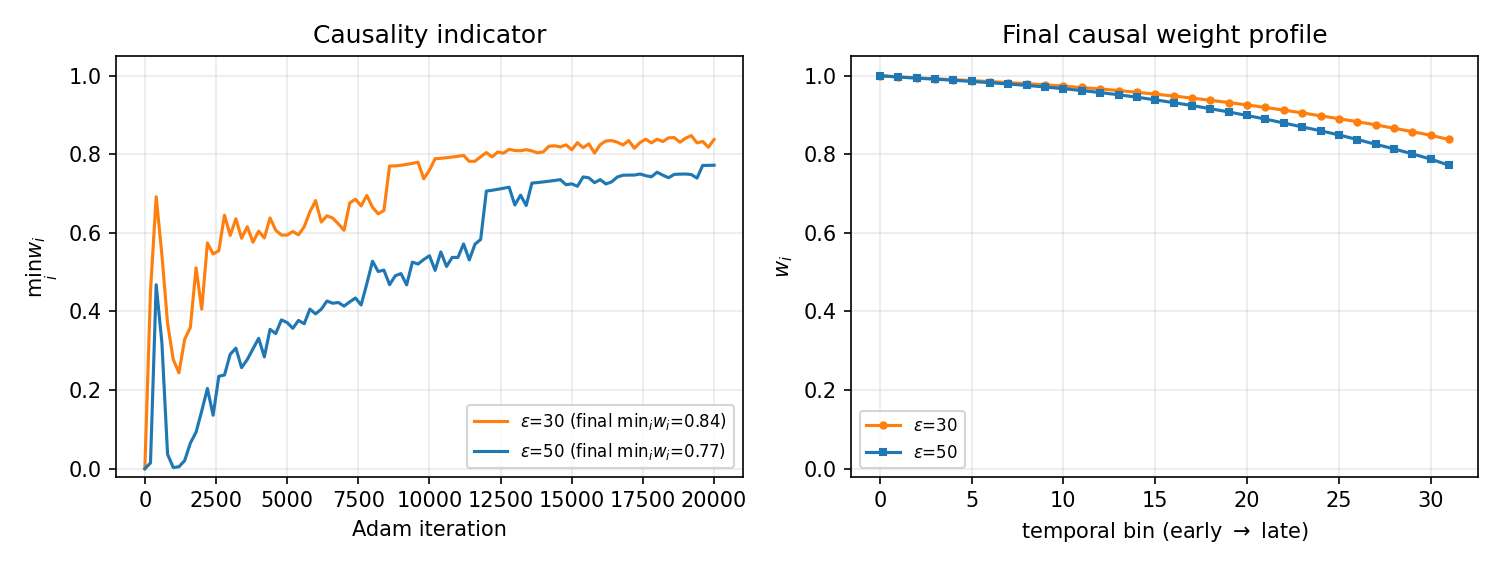
\includegraphics[width=0.78\linewidth]{figures/causal_weight_curve_both.png}
  \caption{Causal curriculum. \emph{Left}: minimum bin weight $\min_i w_i$ versus Adam iteration, saturating at $0.84$ ($\epsilon{=}30$) and $0.77$ ($\epsilon{=}50$) without reaching unity, so the curriculum never fully propagates to the latest bins. \emph{Right}: final weight profiles decrease monotonically from early to late bins, with $\epsilon{=}50$ down-weighting late bins more.}
  \label{fig:causal_weight}
\end{figure}

\begin{figure}[h]
  \centering
  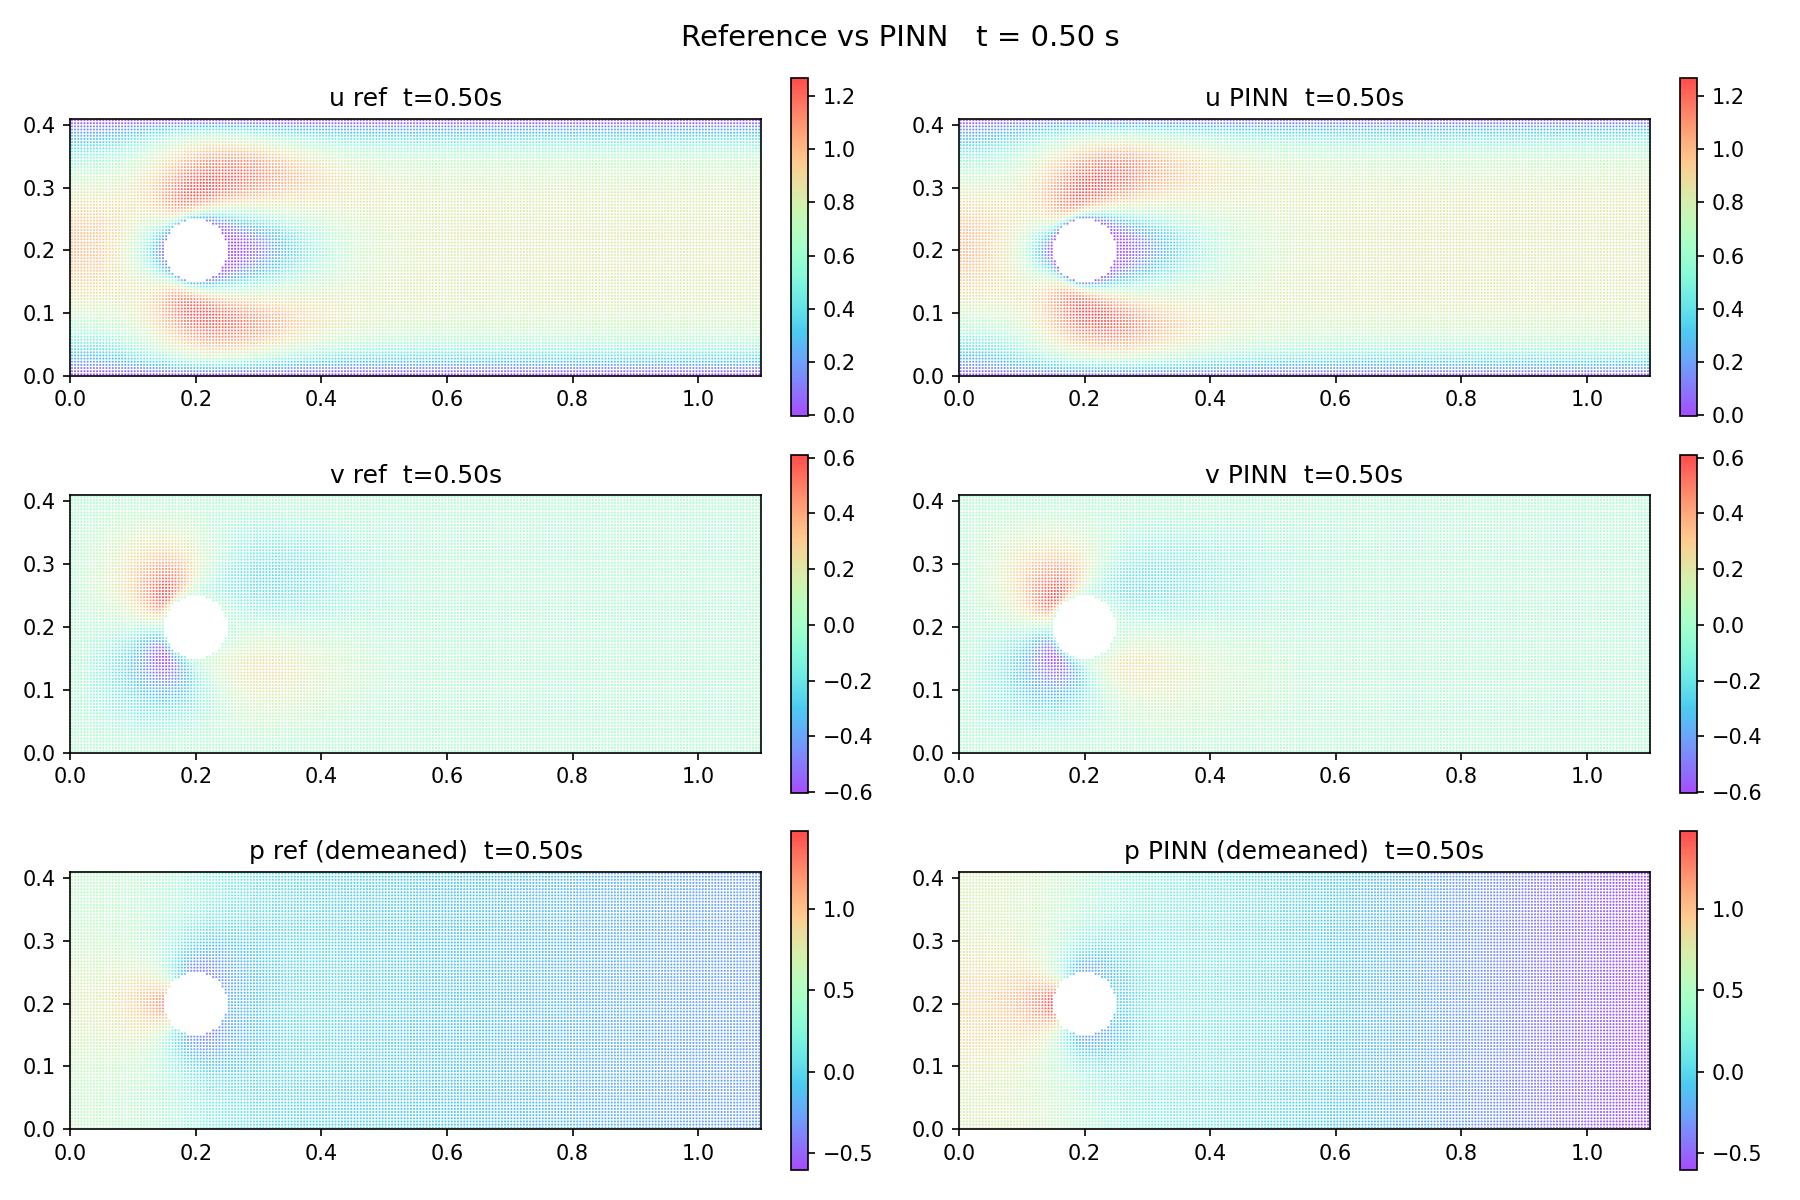
\includegraphics[width=0.72\linewidth]{figures/field_comparison_eps30_uniform_t0p50.png}
  \caption{Reference versus PINN fields at $t=0.5$~s for the best configuration (causal $\epsilon{=}30$, unweighted L-BFGS polish); rows show $u$, $v$, and demeaned $p$. Velocity agrees closely; demeaned pressure recovers the large-scale structure but is the least accurate field.}
  \label{fig:field_comparison}
\end{figure}

\begin{figure}[h]
  \centering
  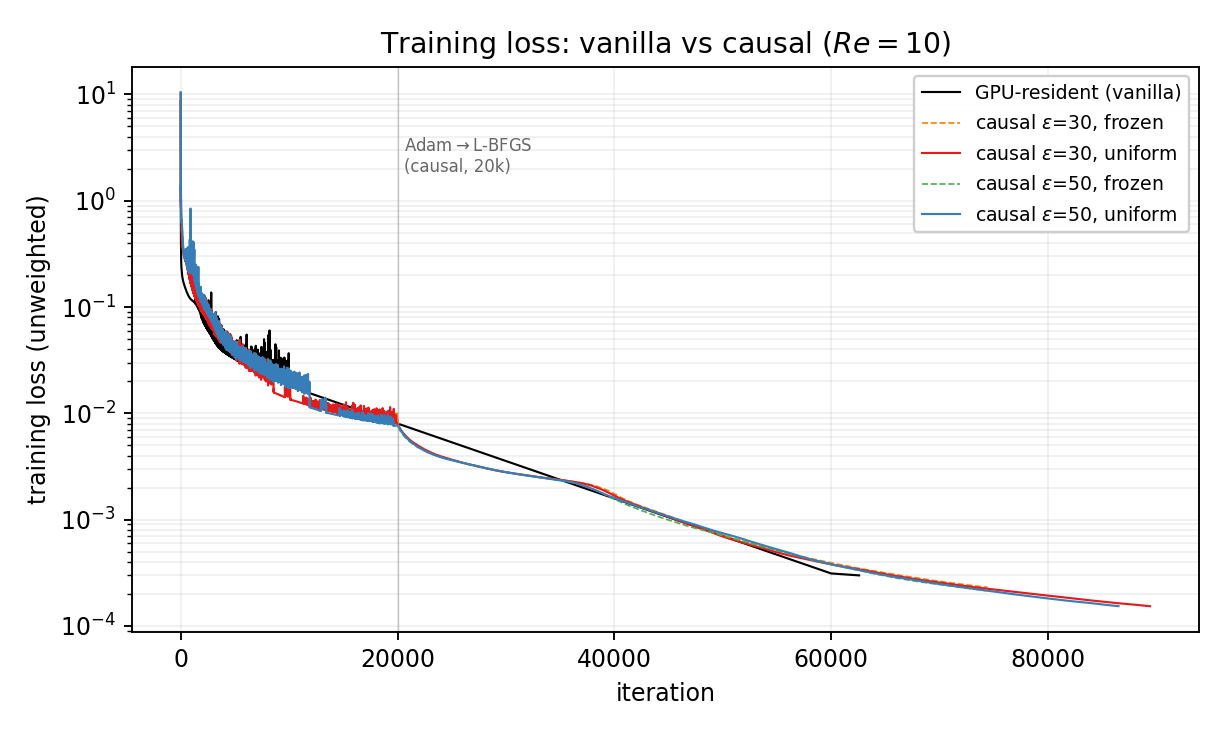
\includegraphics[width=0.7\linewidth]{figures/loss_curves.png}
  \caption{Unweighted training loss versus iteration ($Re=10$, log scale) for the GPU-resident baseline and the four causal runs, all using the Adam$\to$L-BFGS schedule (Adam ends at iteration 20{,}000). The $\epsilon{=}30$ and $\epsilon{=}50$ runs nearly coincide; the uniform-polish variants (solid) reach the lowest final loss.}
  \label{fig:loss_curves}
\end{figure}

\subsection{Model Architecture Variants}

\textcolor{red}{[\textbf{TODO (Chen-Yan Juang)}: discuss the model architecture variants explored, such as SIREN activations~\cite{sitzmann2020siren}.]}

\subsection{3D Extension}
\label{sec:3d}

\textcolor{red}{[\textbf{TODO (Jing-Hua Chang)}: discuss the extension from the 2D formulation to 3D obstacle flow.]}

% --- C2: Discussion merged into Conclusion to compress length; section
% commented out because its content was redundant with the Conclusion.
% Uncomment to restore. ---
\iffalse
\section{Discussion}

The experiments lead to three practical observations. First, the baseline can be reproduced with reasonable agreement, but pressure remains the least stable quantity to evaluate because of gauge sensitivity and projection-reference effects. Second, backend efficiency matters: the GPU-resident implementation improves wall-clock and energy metrics without changing the mathematical objective. Third, the strongest quantitative accuracy improvement comes from training schedule design, especially causality-weighted Adam pretraining followed by unweighted L-BFGS polish. These observations suggest that PINN performance in this benchmark should be analyzed through the interaction between optimizer, sampling distribution, and loss schedule, rather than through the network definition alone.
\fi

\section{Conclusion}

We reproduced the mixed-variable PINN benchmark for $Re=10$ incompressible flow around a cylinder and obtained comparable post-initial-transient accuracy against a Chorin projection reference solution. Our GPU-resident L-BFGS backend reduced wall-clock time by $1.23\times$ and lowered estimated energy by 11.0\% while preserving similar accuracy. Beyond backend efficiency, causality-weighted Adam pretraining followed by unweighted L-BFGS polish achieved the best mean relative $L_2$ errors among our tested configurations (4.64\%, 18.60\%, and 8.89\% for $u$, $v$, and $p$), indicating that temporal loss scheduling can improve PINN optimization.

The main takeaway is that PINN performance for unsteady laminar flow is not determined by the model architecture alone. Backend execution and loss scheduling already show measurable effects on efficiency and accuracy, while adaptive collocation remains a promising sampling mechanism that should be validated with fixed-grid $L_2$ metrics. Future work should integrate adaptive collocation, adaptive loss weighting, and architecture variants into a unified model, and extend the evaluation to higher Reynolds numbers and more complex geometries, building on the preliminary three-dimensional extension outlined in Section~\ref{sec:3d}.

\section{Code and Reproducibility}

The full codebase is available at \url{https://github.com/inQuitiVe/ECE228_PINN}. The main reproduction experiments use the $Re=10$ cylinder-flow benchmark, a Chorin projection reference solution, Adam initialization followed by L-BFGS optimization, and the evaluation metrics defined in Section~\ref{sec:metrics}. The backend benchmark was performed on one RTX 3090 using 1000 controlled L-BFGS function evaluations.

\section{Team Member Contribution}

\begin{itemize}
    \item \textbf{Chi-Han Chiu}: Implemented causal training, GPU-resident L-BFGS benchmarking, core PINN reproduction, and quantitative evaluation.
    \item \textbf{Chen-Yan Juang}: Investigated model architecture variants, including SIREN-style activations, for improving field representation.
    \item \textbf{Ming-Yang Wu}: Developed and tested residual-aware adaptive collocation strategies for sampling.
    \item \textbf{Jing-Hua Chang}: Explored the extension from the baseline 2D formulation to 3D obstacle-flow settings.
\end{itemize}

\bibliographystyle{plain}
\bibliography{reference}

\end{document}
